\chapter{The Super-Kamiokande Detector}
\label{ch:SK_detector}
\graphicspath{{sk_detector/}}
The Super Kamiokande detector is a large water Cherenkov detector in the Gifu, Japan.  In this chapter an overview of the detector apparatus, detection principle, and detector calibration techniques are presented.  Detailed overviews of the detector and detector calibration techniques can also be found in \cite{Fukuda:2002uc} and \cite{Abe:2013gga}.
\section{Overview}
\label{sec:sk_detector_overview}
The SK detector is a large water Cherenkov detector located in the Mozumi mine below Mt. Ikenoyama in Gifu, Japan, with a mean overburden of 1000 m of rock (2700 m water-equivalent.).  It consists of a 50 kT cylindrical tank of water, which is divided into a 32 kT inner detector (ID) surrounded by an 18 kT outer detector (OD).  The ID and the OD are optically separated by black Tyvek sheeting, and both instrumented with photomultiplier tubes (PMTs) to observe Cherenkov radiation. It's large fiducial volume and high quality reconstruction capabilities make it an extremely effective detector for nucleon decay searches and studies of neutrinos over a wide range of energies. \par
The detector's data taking lifetime, which began with it's commissioning  April 1996, is divided into four phases.  The first phase, known as ``SK-I", acquired 1489.2 livetime days of data, running from commissioning until July 2001, when the detector was shut down for maintenance and upgrades.  During the refilling of the tank in November 2001, and accident destroyed over half of the ID PMTs.  The remaining ID PMTs were fitted with protective cases to avoid a future accident and redistributed, and the second phase, known as ``SK-II", ran from October 2002 until October 2005 with only half the ID PMT coverage of SK-I, acquiring 798.6 livetime days of data.  During the shutdown after SK-II, new ID PMTs were added, and data taking resumed in July 2006 with the ID PMT coverage back at SK-I levels.  This third phase is known as ``SK-III", and acquired 518.1 livetime days of data, running until September 2008, when the experiment was briefly shutdown for an electronics upgrade.  Upon restarting in September 2008 SK entered it's fourth phase, known as ``SK-IV", which is ongoing as of the writing of this thesis, and which has acquired 2867.2 livetime days of data as of May 2017.  In total, SK has recorded 5673.1 livetime days of data (as of May 2017) with just over half of that data coming during SK-IV.      
\section{The Tank}
\label{sec:tank}
The main component of the SK detector is a cylindrical stainless steel tank, with a diameter of 39 m and a height of 42 m, which is filled with about 50 ktons of water.  The structure of the detector is shown in \cref{fig:sk_detector_diagrams}.  The tank is segmented into an inner detector (ID), with a diameter 33.8 m and a height of 36.2 m, which hold 32 ktons of water, and an outer detector (OD) which is the region of the tank outside the ID.  The ID is the primary detector used for most physics analyses, while the OD is primarily used as an active cosmic ray veto.  The ID and OD are separated from one another by a cylindrical PMT support structure.  On the inner surface of the support structure, 11,146 inward-facing 20 inch PMTs, giving a coverage of about 40\% are mounted to observe activity in the ID (for SK-II half as many PMTs were used in the ID).  The outer surface of the support structure is instrumented with 1885 outward-facing 8 inch PMTs to observe the OD.  Lightproof Tyvek sheeting on both surfaces of the PMT structure optically separates the ID from the OD.  It also results in a 55 cm this dead space between the ID and the OD, from which light cannot escape.  The Tyvek sheeting is black on the side facing into the ID, in order to reduce reflections which would diminish reconstruction accuracy.  On the side facing the OD, conversely, the Tyvek sheeting is white, in order to increase reflections.  This is done to improve light collection efficiency in the OD, the compensate for its lower PMT coverage.  Scattered light in the OD is also much less problematic for physics goals compared to scattered light in the ID. \par
The PMTs are very sensitive to magnetic fields, and the about 450 mG geomagnetic field at the SK detector site would significantly reduce their efficiency.  Therefore, 26 sets of horizontal and verticle Helmholtz coils are arranged around the inner surface of the tank.  These reduce the magnetic field in the tank to about 50 mG, which results in an estimated about 1-2\% effect on the collection efficiency of the ID PMTs. 

\begin{figure*}
\centering
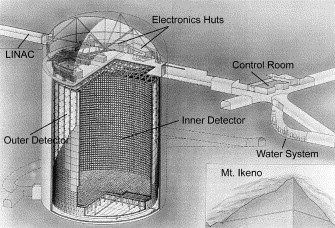
\includegraphics[width=0.8\textwidth]{figures/sk_detector_under_mountain.jpg}
\caption{Structure of the SK detector. \cite{Fukuda:2002uc}}
\label{fig:sk_detector_diagrams} 
\end{figure*}

\begin{figure*}
\centering
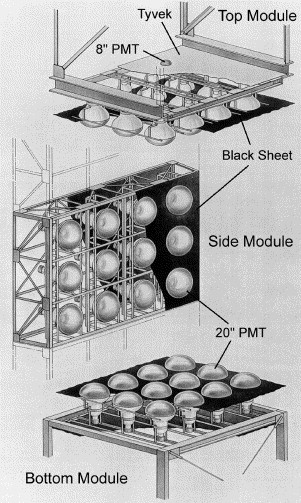
\includegraphics[width=0.8\textwidth]{figures/pmt_support_structure.jpg}
\caption{PMT support structure. \cite{Fukuda:2002uc}}
\label{fig:pmt_support_structure} 
\end{figure*}
\section{Cherenkov Radiation}
\label{ch:cherenkov_radtion}
When a charged particle travels through a material at a speed faster than the phase velocity of light in the material, Cherenkov radiation is produced.  Molecules excited by the particle release light, and when the particle is traveling faster than $c/n$, the light emitted from different points along the particles path interferes constructively to create Cherenkov radiation, as shown in \cref{fig:cherenkovradiation}.  The requirement for Cherenkov radiation is thus
\begin{equation}
\beta>\frac{1}{n}.
\label{eq:cherenkov_req}
\end{equation}
The Cherenkov radiation is emitted from the path of the charged particle along a cone centered on the path of the charged particle with half opening angle $\theta_C$ given by:
\begin{equation}
\cos \theta_C=\frac{1}{\beta n}.
\label{eq:cherenkov_angle}
\end{equation}
A detailed derivation of these formula based on electrodynamics can be found in \cite{Jackson:1998nia}.
\begin{figure}
\centering
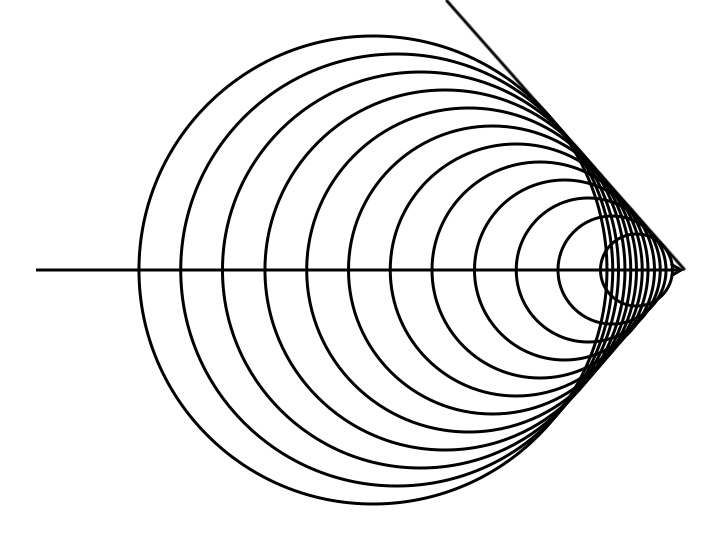
\includegraphics[width=0.8\textwidth]{figures/Cherenkov_radiation.png}
\caption{Constructive interference resulting in Cherenkov radiation.}
\label{fig:cherenkovradiation}
\end{figure}
The index of refraction of water is 1.34, so for charged particles in water the cherenkov threshold corresponds to $\beta>0.75$.  This can be translated to a momentum threshold of $p>1.13m$, which equates to a momentum threshold of 577 KeV/c for electrons, 119 MeV/c for muons, 157 MeV/c for charged pions, and 1.058 GeV/c for protons.  The cherenkov angle for a highly relativistic charge particle in water ($\gamma \gg 1$) of about 42$^\circ$.  \par
The emitted spectrum is described by the formula\cite{Olive:2016xmw}:
 \begin{equation}
\frac{d^2N}{d\lambda dx}=\frac{2\pi \alpha z^2}{\lambda^2}\left(1-\frac{1}{\beta^2\n^2(\lambda)}\right)
\label{eq:cherenkov_spectrum}
\end{equation}
where $\alpha$ is the fine structure constant, $z$ is the charge of the particle (in units of electron charge), $\lambda$ is the wavelength of the emitted light, and $x$ is the distance traveled by the charged particle.  It should be noted that whil this formula allows for a wavelength dependent index of refraction, the index of refraction of water is quite stable of the range of wavelengths observed by PMTs.   

\section{Photomultiplier Tubes}
\label{sec:pmts}
The ID PMTs are 20-inch PMTs (Hamamatsu R3600) built by Hamamatsu Photonics K.K.  A schematic is shown in \cref{fig:pmt}  These PMTs were based off an earlier Hamamtsu designed 20-inch PMT (Hamamatsu R1449) which had been used in the Kamiokande Detector.  The Kamiokande design was improved upon in collaboration with Hamamatsu for use in Super-Kamiokande \cite{Suzuki:1992as}.  The photocathode is made of bialkali, which was chosen for its high sensitivity to blue light and low thermionic emission.  The quantum efficiency of the photocathode peaks around 21\% between 360 and 400 nm, and is shown as a function of wavelength along with the emitted spectrum of Cherenkov light in water in \cref{fig:pmt_qe_cherenkov_spectrum}. The dynode structure is a venitian blind type, which was optimized to improve photoelectron (p.e.) timing resolution and collection efficiency \cite{Suzuki:1992as}.  The single p.e. pulse height distribution and transit time distribution are shown in \cref{fig:pmt_pe_and_timing}.\par    

\begin{figure}
\centering
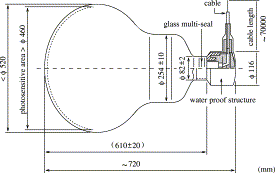
\includegraphics[width=0.8\textwidth]{figures/pmt.png}
\caption{Schematic of the ID PMTs. \cite{Fukuda:2002uc}}
\label{fig:pmt}
\end{figure}

\begin{figure}
\centering
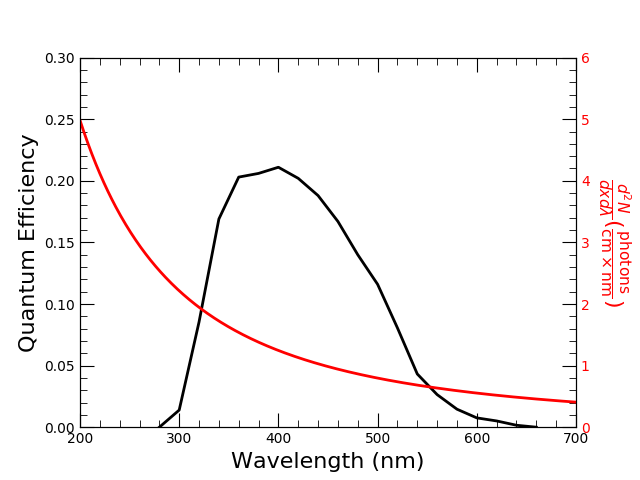
\includegraphics[width=0.8\textwidth]{figures/pmt_qe_cherenkov_spectrum.png}
\caption{Photocathode quantum efficiency in black and emitted Cherenkov spectrum in red.  Note different y-axes.}
\label{fig:pmt_qe_cherenkov_spectrum}
\end{figure}

\begin{figure}
\centering
\subfigure[]{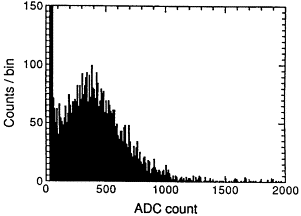
\includegraphics[width=0.4\textwidth]{figures/pmt_single_pe.png}
\label{fig:pmt_1pe_pusle_height}	
}
\subfigure[]{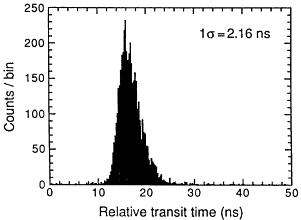
\includegraphics[width=0.4\textwidth]{figures/pmt_transit_time.png}
\label{fig:pmt_transit_time}	
}
\caption{Left: ID PMT single p.e. pulse height distribution.  The peak near zero ADC counts is the result of dark current.  Right: ID PMT relative transit time distribution at 410 nm and single p.e. level.  Both from \cite{Fukuda:2002uc}}
\label{fig:pmt_pe_and_timing}
\end{figure}

In order to prevent another accident like the one which occurred during upgrade work after SK-I, all PMTs have been enclosed in a protective case since the beginning of SK-II.  These protective cases consist of an acrylic dome over the face of the PMT, and a fiber-reinforced plastic (FRP) case around the sides and back of the PMT.  The FRP case has holes in it which allow water to flow freely around the PMT, but also restrict the speed with which water can rush into the vacuum of a PMT in case of a PMT implosion.  This mitigates the creation of a shock wave, which was determined to be the cause of the original accident.  \par

The OD PMTs are 8-inch PMTs, also produced by Hamamatsu.  Five-hundred ninety-one are old Hamamatsu R1408 PMTs, recycled form the IMB experiment, which 1293 are new Hamamatsu R5912 PMTs, installed during the upgrades between SK-I and SK-II, and SK-II and SK-III.  The single p.e. distributions for the old and new tubes are shown in \cref{fig:od_1pe}.

\begin{figure}
\centering
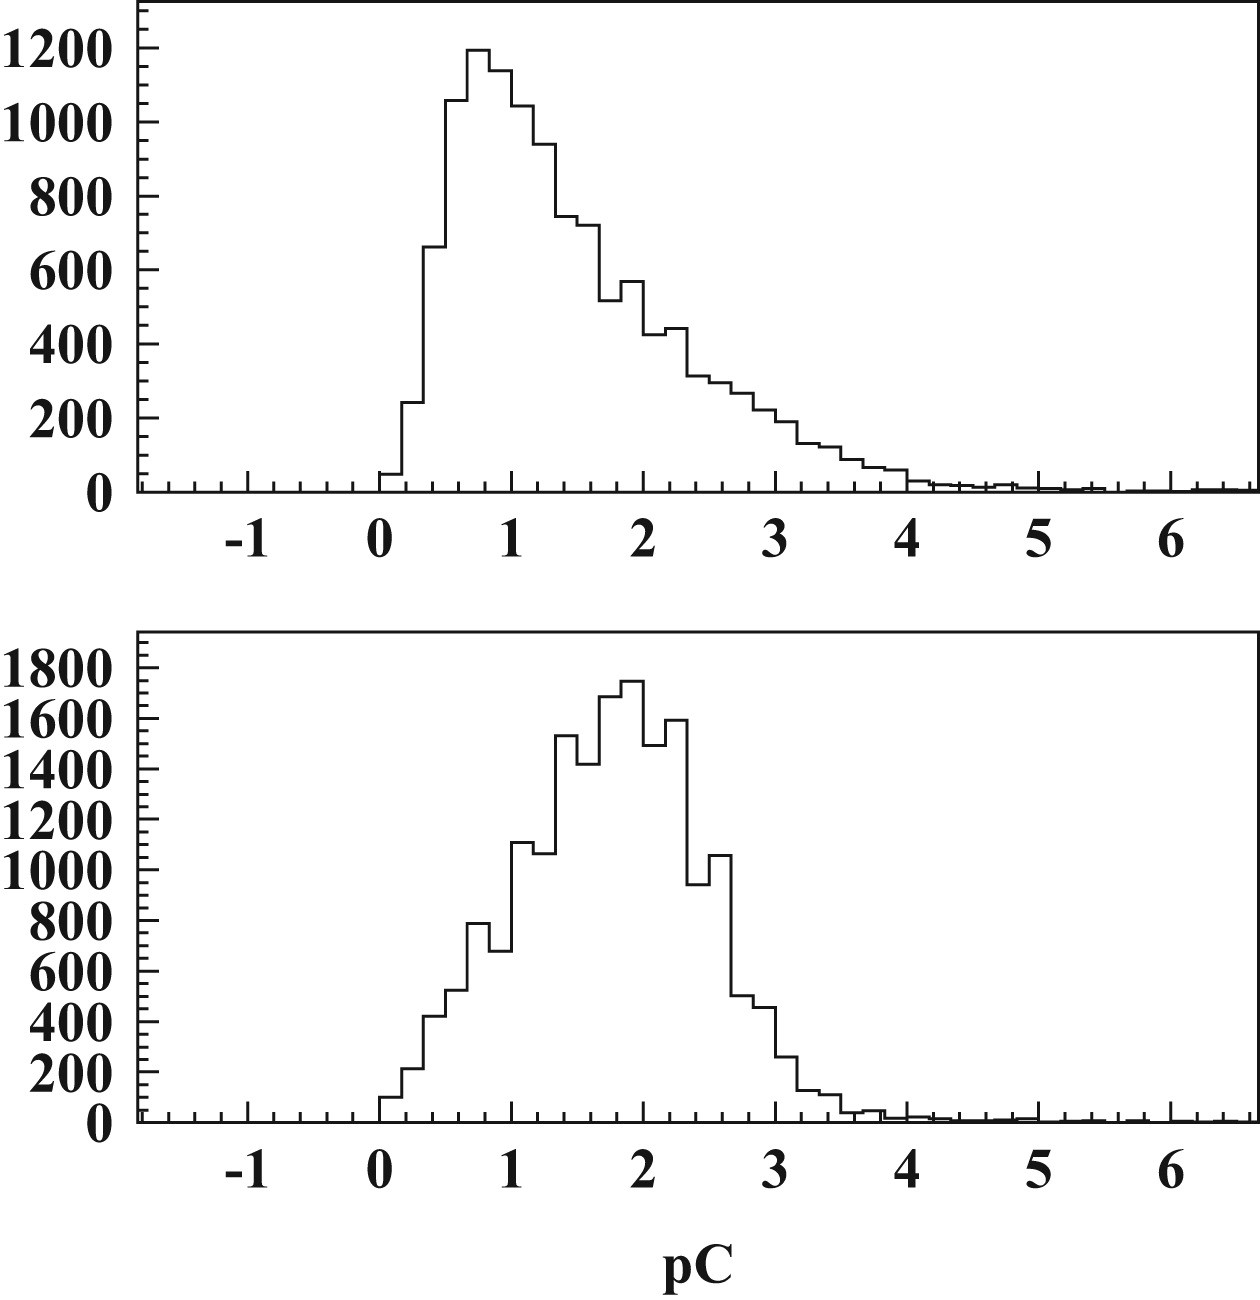
\includegraphics{figures/OD_1pe_distribution.jpg}
\caption{Top: Single p.e. distribution of OD old PMTs (Top) and new PMTs (Bottom).}
\label{fig:od_1pe}
\end{figure}
 
\section{Electronics and Data Acquisition}
\label{sec:daq}
The SK Electronics and Data Acquisition System (DAQ) was extensively upgraded between SK-III and SK-IV.  As such, the SK-IV electronics will be explained separately from the SK I-III electronics.
\subsection{SK I-III}
\label{subsec:sk_1_3_daq}
The SK I-III DAQ processed ID PMT signals using custom build Analog-Timing-Modules (ATMs), which were originally designed and built by KEK.   A schematic of the ATM can be seen in \cref{fig:daq_ATM}  The PMT signal was split into four signals.  One of these signals was sent to a discriminator, which compared the signal to a threshold corresponding to 1/4 pe equivalent.  When the signal crossed this threshold, a 200ns wide logic pulse was sent to a hardware trigger module.  Simultaneously, the signal from the PMT was stored by a Charge-to-Analog Converter (QAC), and a integration of a constant current was started by a Time-to-Analog Converter (TAC).  When a global trigger was received from the hardware trigger module, the TAC integration was stopped and the information in the QAC and TAC were sent to and Analog-to-Digital Converter (ADC) to be digitized and stored in internal memory.  Because the TAC integrated a constant charge from the time of the channel trigger to the time of the global trigger, the time of the PMT signal relative to the global trigger can be calculated from the total integrated charge on the TAC.  Each channel was assigned two TACs and QACs, in order to process events which might occur in rapid succession, such as the a decay electron following a muon.  The charge dynamic range of the ATM was about 450 pC, with a resolution of 0.2 pC, while the timing dynamic range was 1.3 $\mu$s, with a resolution of 0.4 ns.\par
A hitsum was calculated by the hardware trigger module by simple analog sum of the logic signals from the ATMs.  When the hitsum crossed a given threshold, a global trigger would be issued to the ATMs.  Three different triggers were used: high energy (HE), low energy (LE) and super low energy (SLE).  The HE and LE triggers were set at 31 and 29 hits, respectively, with the LE threshold corresponding to an electron energy of 5.7 MeV.  The SLE trigger was added to lower the energy threshold to 4.6 MeV.  The trigger logic and interaction with the ATMs is shown in \cref{fig:daq_trigger_1_3}, and a full schematic of the DAQ is shown in         
\cref{fig:daq_schematic_1_3}.  The OD operated with a similar trigger system, and OD triggers were issued with a threshold of 19 hits.  Additional details of the ID and OD electronics and DAQ for SK I-III can be found in \cite{Fukuda:2002uc}. 
\begin{figure}
\centering
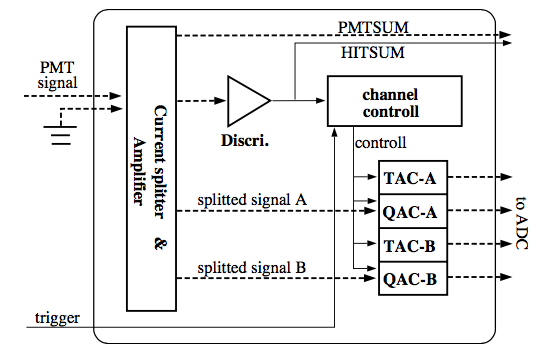
\includegraphics[width=0.5\textwidth]{figures/SK_1_3_ATM.png}
\caption{Schematic of processing of one channel by the ATM, used in SK I-III.  Dashed lines represent analog signals while solid lines represent logic signals \cite{Fukuda:2002uc}.}
\label{fig:daq_ATM}
\end{figure}

\begin{figure}
\centering
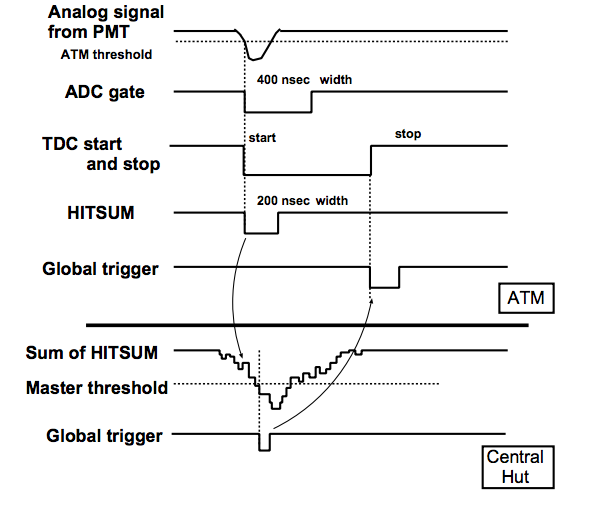
\includegraphics[width=0.5\textwidth]{figures/ID_trigger_SK1_3_Nishino.png}
\caption{Trigger system used in SK I-III \cite{Nishino:2009lps}.}
\label{fig:daq_trigger_1_3}
\end{figure}

\begin{figure}
\centering
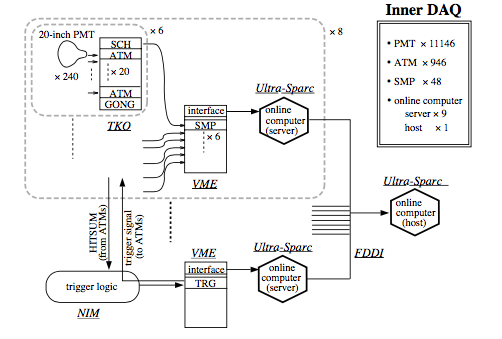
\includegraphics[width=0.5\textwidth]{figures/SK_1_3_daq.png}
\caption{Schematic of SK I-III DAQ.  Lines indicate flow of data \cite{Fukuda:2002uc}.}
\label{fig:daq_schematic_1_3}
\end{figure}

\subsection{SK-IV}
\label{subsec:sk_4_daq}
As mentioned earlier, the SK electronics were upgraded between SK-III and SK-IV \cite{Yamada:2010zzc,Nishino:2009zu}.  The ATM was replaced by a front end electronics board called a QBEE, which stands for "QTC (Charge-to-Time Converter) Based Electronics with Ethernet."   A QBEE is shown in \cref{fig:QBEE}.  PMT signals are processed by a QTC, which encodes the time and charge of the PMT pulse into the timing of a single pulse, as shown in \cref{fig:QTC_timing}.  When the PMT signal crosses a threshold which corresponds to about 1/4 pe (the same as in SK I-III), the QTC begins an output pulse, and a capacitor charges up over 400 ns with the charge from the PMT pulse.  The capacitor is then discharged at a constant rate, and the QTC output pulse is stopped when the capacitor charge drops below a comparator level.  The QTC output pulse thus encodes the time of the PMT pulse as the time of its leading edge, and the charge of the PMT pulse as its width. This full encoding and processing results in a deadtime of 900 ns.\par
Each PMT signal is processed by a QTC under three different gain settings, called ``Small", ``Medium" and ``Large", with gain ratios 1:$\frac{1}{7}$:$\frac{1}{49}$.  The charge dynamic ranges of the three gain setting are shown in \cref{tab:QTC_dynamic_ranges}.  While each PMT signal is process under all three gain settings, only the result from the lowest gain setting which is not saturated is used.  This results in a charge resolution similar to the ATMs used in SK I-III, but with about five times the dynamic range.\par   
The hardware trigger used in SK I-III is replaced by a software trigger for SK-IV.  Every hit recorded by the QBEEs is sent to Front-End PCs, with each Front-End PC receiving the hits from 30 QBEEs.  The data from the Front-End PCs is the sent on to Merger PCs, which combine the hits from all PMTs and apply software triggers to search for physics events.  When a software trigger is generated, the event data is sent to an Organizer PC, which writes the data onto disk for offline analysis.  This data flow is visualized in \cref{fig:sk_4_data_flow}.\par
The software trigger of SK-IV has multiple advantages over the hardware trigger of SK-III.  Primarily, it allows for any length of event, more complex trigger logic, and easy introduction of new triggers.  The main triggers used in SK-IV are summarized in \cref{tab:triggertable4}.  While the SLE, HE, SHE, and OD triggers perform functionality achievable which the SK I-III hardware trigger, the AFT trigger shows the true power of moving to a software trigger for SK-IV.  The AFT trigger is used for tagging neutrons, which capture and produce a 2.2 MeV $\gamma$ on the order of hundreds of $\mu$s after a primary neutrino event.  They do not produce enough hits to generate an SK I-III hitsum trigger, and lowering the hitsum threshold to catch such events would result in an significantly increased data rate and require substantially more computing power and disk space to handle.  This means that neutron tagging is impossible in SK I-III.  The software trigger of SK-IV solves all of these problems with the AFT trigger, which takes advantage of both the complex trigger logic and variable event width available in the software trigger system.    

\begin{table}
\centering
	\begin{tabular}{lcc}
	\hline \hline
	Gain Setting&Dynamic Range&Resolution\\
	\hline
	Low&51 pC&0.1 pC\\
	Medium&357 pC&0.7 pC\\
	High&2500 pC& 4.9 pC\\
   \hline \hline
	\end{tabular}
\caption{Charge dynamic ranges for the three gain settings of the SK-IV QTC.}
\label{tab:QTC_dynamic_ranges}
\end{table}

\begin{table}[!ht]
\centering
\begin{tabular}{lcccc}
\hline \hline
SK-IV Triggers & Trigger Logic & Event Width ($\mu s$) \\
\hline
SLE & 34 (31) hits in 200 ns & -0.5$\rightarrow$ 1.0 \\
HE & 50 hits in 200 ns & -5$\rightarrow$ 35 \\
SHE & 70 (58) hits in 200 ns & -5$\rightarrow$ 35\\
OD & 22 hits in 200 ns (in OD) & \\
AFT & SHE, no OD & 35 $\rightarrow$ 535 \\
\hline \hline
\end{tabular}
\caption{Trigger information for SK-IV. The abbreviations are as follows: 
OD (outer detector), SLE (super low energy), HE (high energy), SHE (
special high energy) and AFT (after).  The SLE and SHE trigger thresholds were lowered from 34 to 31 and 70 to 58 hits respectively, during SK-IV running.  There are $\sim$9 hits of dark noise 
in 200~ns and $\sim$6 hits corresponds to 1 MeV electron equivalent energy.}
\label{tab:triggertable4}
\end{table}

\begin{figure}
\centering
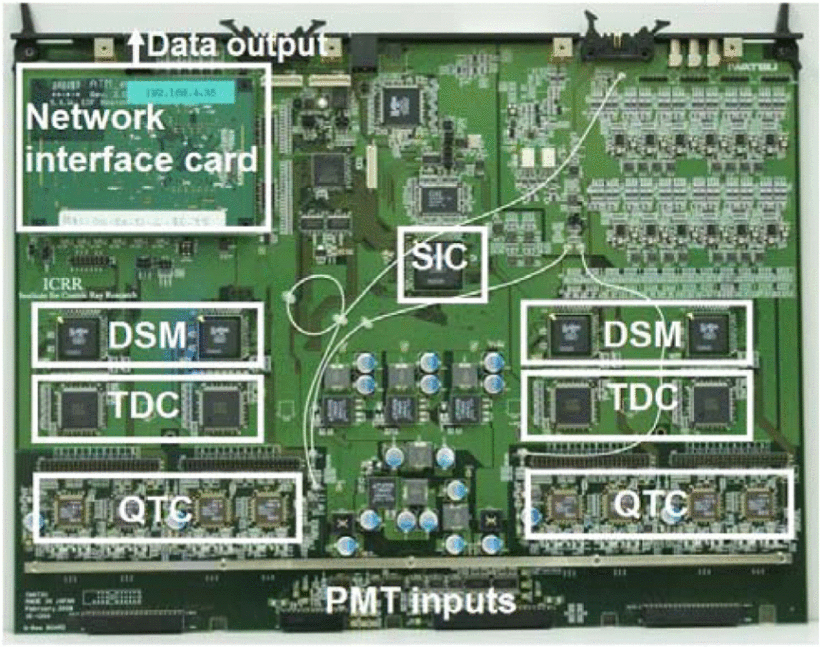
\includegraphics[width=0.5\textwidth]{figures/QBEE.png}
\caption{Front end electronics used in SK-IV, called QBEE \cite{Yamada:2010zzc}}
\label{fig:QBEE}
\end{figure}      

\begin{figure}
\centering
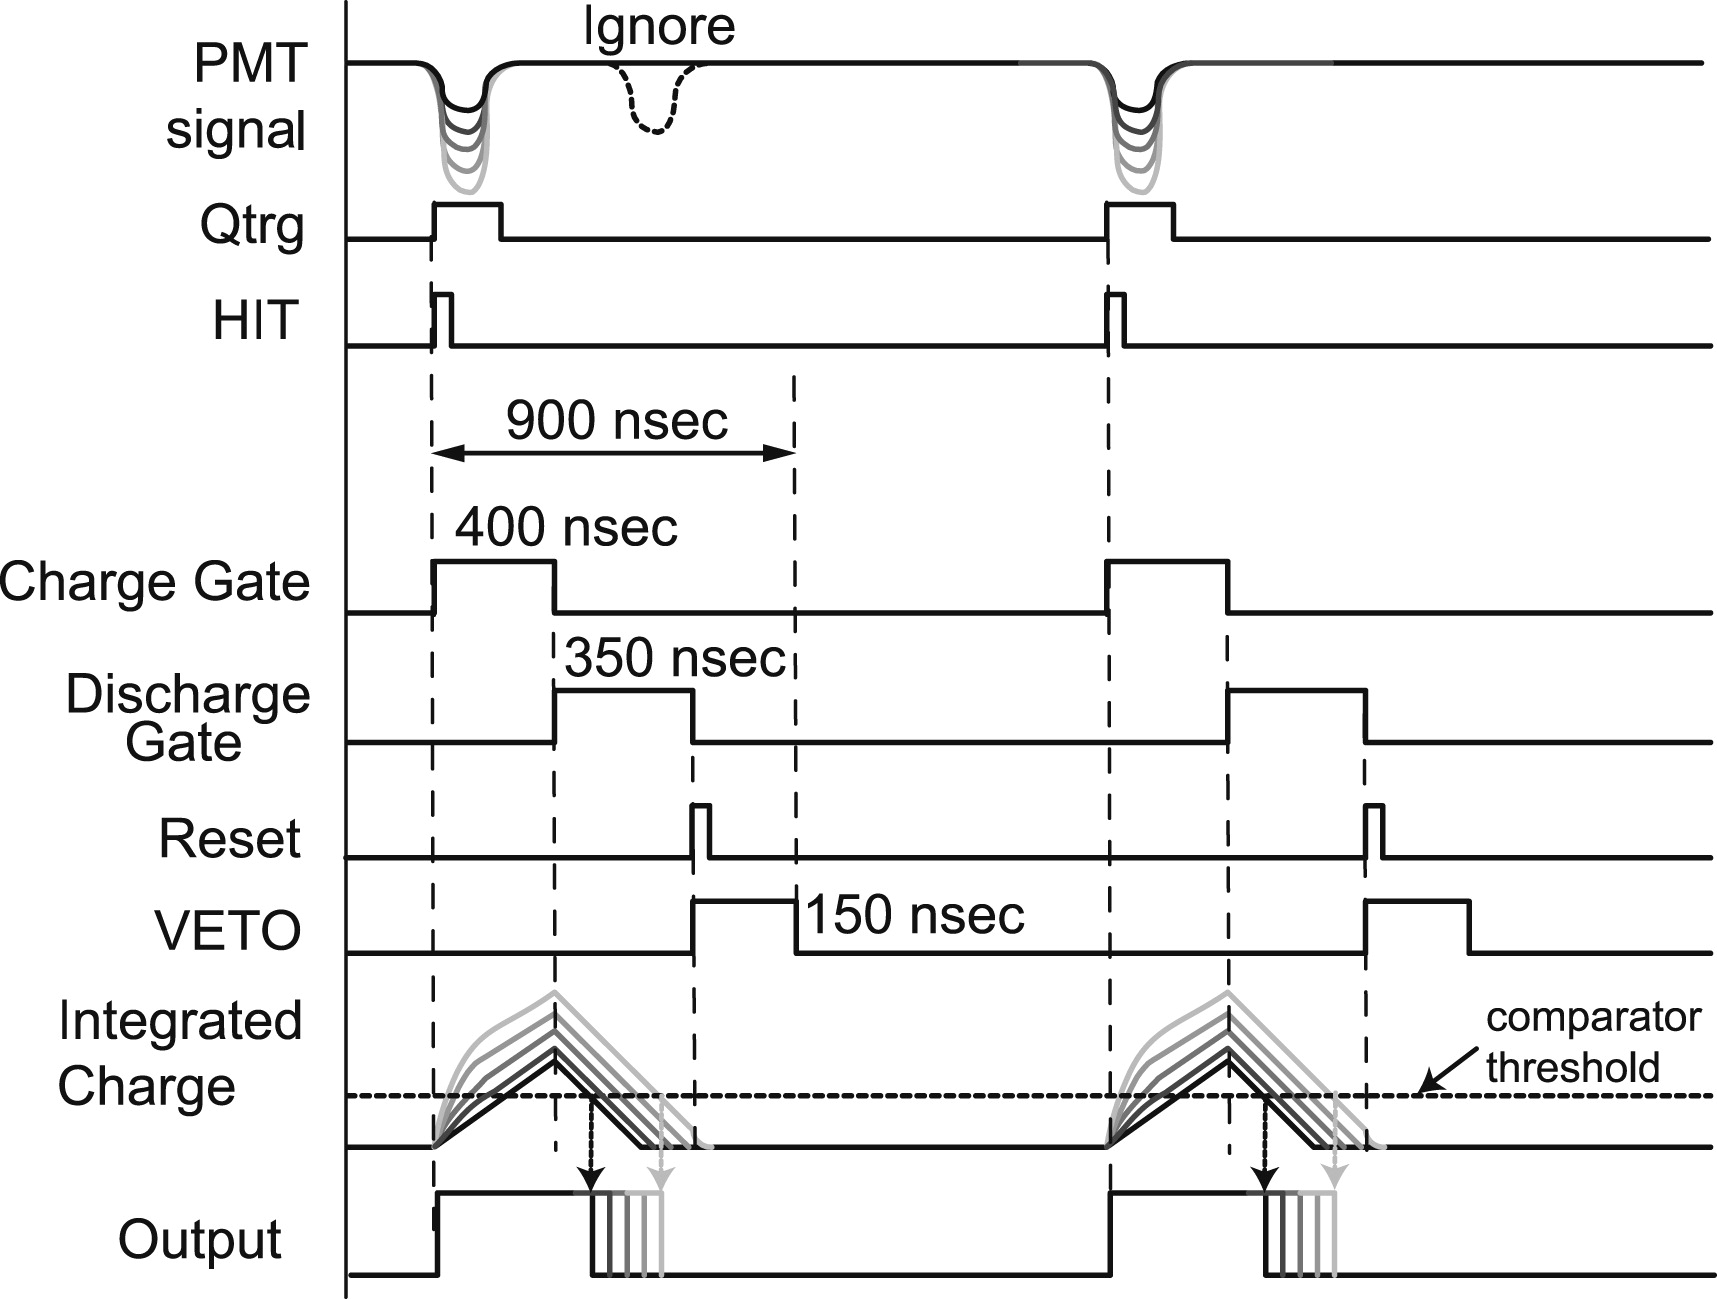
\includegraphics[width=0.5\textwidth]{figures/QTC_timing.jpg}
\caption{QTC charge and time encoding for QBEE \cite{Nishino:2009zu}.}
\label{fig:QTC_timing}
\end{figure}    

\begin{figure}
\centering
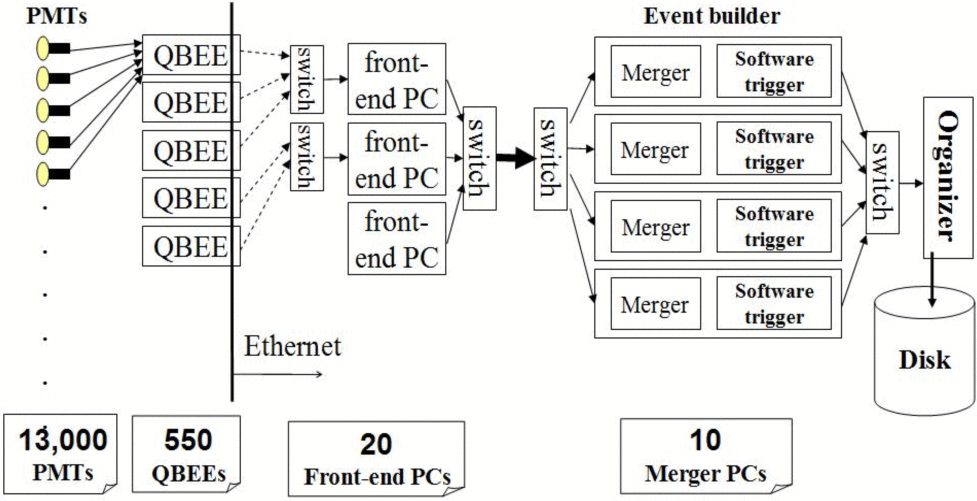
\includegraphics[width=0.5\textwidth]{figures/SK_4_data_flow.png}
\caption{SK-IV data flow \cite{Yamada:2010zzc}}
\label{fig:sk_4_data_flow}
\end{figure} 
\section{Water System}
\label{sec:water_system}
 
\section{Detector Calibration}
\label{sec:calibration}